\contribution{The Bus}
\shortcontributor{CS6230 : CAD for VLSI Project Report}
\shortcontribution{Overview}
\headnum{4}
\begin{paper}
\renewcommand*{\pagemark}{}

\section*{}
Although Bluespec provides a Config bus (CBus) interface through the CBus and LBus package, top-level test benches have to be written to mediate communication between two or more module interfaces. Employing the CBus package hindered modularity as we insisted our modules to have plug and play interfaces. Bluespec also had implemented in their libraries many of the standard bus protocols like AHB and AXI with TLM interface. These provided full-fledged capabilities that were overkill for use in our system. So, we decided on a simple bus protocol to implement ourselves on Bluespec.
\section*{The Bus System\sdot}
\begin{figure}[H]
\centering
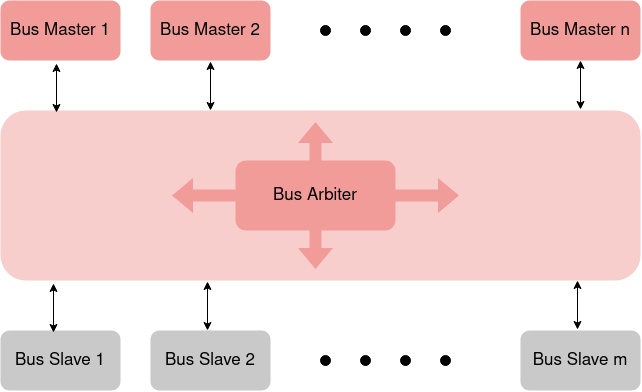
\includegraphics[width=8cm]{Images/Overview-Bus.png}
\caption{\content The bus system.}
\end{figure}\\
\nointend The system consists of a Bus Fabric to which different modules are connected. There are two types of modules, the Bus Masters and the Bus Slaves. Masters issue read or write requests to which slaves have to respond if the requested address is within its scope. The bus Arbiter determines which master owns the bus. Before sending a request, all masters must request the Arbiter. In the case of multiple requests, the Arbiter uses round-robin scheduling to select the owner of the bus. We used Bluespec's \texttt{Arbiter} package for implementing the Arbiter.
\section*{The Bus Protocol\sdot}
\begin{figure}[H]
\centering
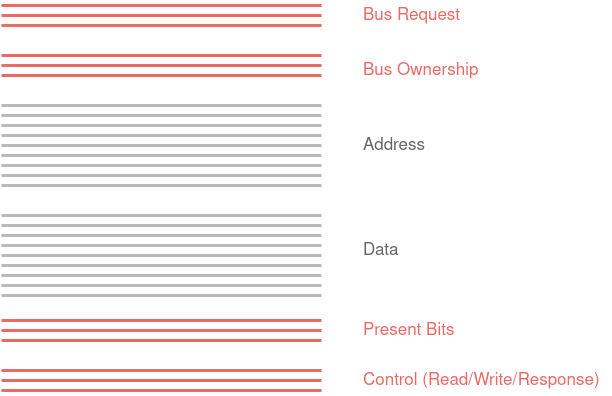
\includegraphics[width=8cm]{Images/Overview-BusWires.png}
\caption{\content The bus wires.}
\end{figure}\\
\nointend Every master gets assigned two exclusive lines, one for requesting the Arbiter and another to receive the Arbiter response. All the rest of the Bus lines are shared.\\\\
\nointend A read request consists of an Address, the present bits indicating the number of units of the smallest addressable blocks expected by the sender, and the control wires in 'Read' mode. For example, to request four consecutive bytes to a RAM whose smallest addressable unit is 1 byte, we have our present bits to have a value of 4. In this way, connected slaves can utilize the entire bus width to the maximum. Similarly, a write request consists of almost the same details except for the data and control in 'Write' mode. Slaves respond with the appropriate 'Response.'
\section*{Interfacing the Bus\sdot}
The BusMaster and BusSlave modules provide an effortless bridge between the Bus and the associated components. Read/write requests can be enqueued into the BusMaster, and responses can be read using simple GetPut interfaces. Corresponding interfaces also exist towards the BusSlaves.
\begin{figure}[H]
\centering
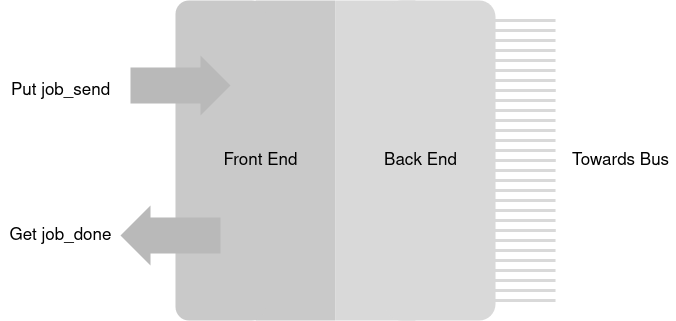
\includegraphics[width=8.8cm]{Images/Overview-BusMaster.png}
\caption{\content The BusMaster.}
\end{figure}
\begin{figure}[H]
\centering
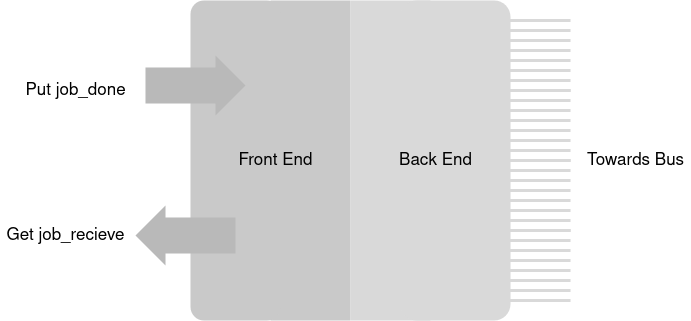
\includegraphics[width=9cm]{Images/Overview-BusSlave.png}
\caption{\content The BusSlave.}
\end{figure}\\
\nointend For details about using the Bus, see the documentation section.
\end{paper}